% questions.tex —— 2009 年·普通高等学校招生考试·福建卷·文科 · 题目内容片段（无答案）
% 由 tools/generate_projects.py 依来源总账自 2009/2009_数学真题_福建文_试题.md 生成，勿手改（改源 MD 后重跑）


状态：needs-review；依固定候选 PDF 两页（印刷页 517–518）逐题核验，四幅图已矢量重绘。原页未印分值，不补。

\gkpart{一、选择题}

\begin{question}
\gkti{1}若集合 $A=\{x\mid x>0\}$，$B=\{x\mid x<3\}$，则 $A\cap B$ 等于（　）

（A）$\{x\mid x<0\}$

（B）$\{x\mid 0<x<3\}$

（C）$\{x\mid x>3\}$

（D）$\mathbf R$

\end{question}
\begin{question}
\gkti{2}下列函数中，与函数 $y=\dfrac1{\sqrt x}$ 有相同定义域的是（　）

（A）$f(x)=\ln x$

（B）$f(x)=\dfrac1x$

（C）$f(x)=|x|$

（D）$f(x)=\mathrm e^x$

\end{question}
\begin{question}
\gkti{3}一个容量 $100$ 的样本，其数据的分组与各组的频数如下表

\begin{center}
\begingroup\setlength{\tabcolsep}{4pt}
\begin{tabular}{llllllll}
\toprule
组别 & $(0,10]$ & $(10,20]$ & $(20,30)$ & $(30,40)$ & $(40,50]$ & $(50,60]$ & $(60,70]$ \\
\midrule
频数 & $12$ & $13$ & $24$ & $15$ & $16$ & $13$ & $7$ \\
\bottomrule
\end{tabular}
\endgroup
\end{center}

则样本数据落在 $(10,40)$ 上的频率为（　）

（A）$0.13$

（B）$0.39$

（C）$0.52$

（D）$0.64$

\end{question}
\begin{question}
\gkti{4}若双曲线 $\dfrac{x^2}{a^2}-\dfrac{y^2}{3^2}=1$（$a>0$）的离心率为 $2$，则 $a$ 等于（　）

（A）$2$

（B）$\sqrt3$

（C）$\dfrac32$

（D）$1$

\Needspace{0.4\textheight}
\end{question}
\begingroup
\renewenvironment{question}{\Needspace{0.5\textheight}}{}
\begin{question}
\gkti{5}如图，某几何体的正视图与侧视图都是边长为 $1$ 的正方形，且体积为 $\dfrac12$．则该几何体的俯视图可以是（　）
\nopagebreak[4]
\begin{center}% 2009 年福建卷文科第 5 题：四个俯视图选项（A）—（D）。
% 来源 PDF：普通高考/2009/2009福建文.pdf，SHA-256 f0a5111a6f86f4d4e8618c5c2cd0ecfd678a590b36ecbd033bb63b189700a0bc。
% 原页：第 1 页（A3 三栏）第 1 栏下部，书页码 517。
% 重绘依据：按原页四幅小图重绘；A 正方形、B 圆、C 等腰直角三角形、D 四分之一圆。
\begin{tikzpicture}[semithick, every node/.style={inner sep=1.4pt, font=\small}]
  % A：正方形
  \draw (0,0) rectangle (1.2,1.2);
  \node[below] at (0.6,-0.15) {（A）};
  % B：圆
  \draw (2.6,0.6) circle (0.6);
  \node[below] at (2.6,-0.15) {（B）};
  % C：等腰直角三角形
  \draw (4.0,0) -- (5.2,0) -- (4.0,1.2) -- cycle;
  \node[below] at (4.6,-0.15) {（C）};
  % D：四分之一圆
  \draw (6.2,0) -- (7.4,0) arc (0:90:1.2) -- cycle;
  \node[below] at (6.8,-0.15) {（D）};
\end{tikzpicture}
\end{center}
\nopagebreak[4]
\Needspace{0.4\textheight}
\end{question}
\endgroup
\begingroup
\renewenvironment{question}{\Needspace{0.5\textheight}}{}
\begin{question}
\gkti{6}阅读如图所示的程序框图，运行相应的程序，输出的结果是（　）
\nopagebreak[4]
\begin{center}% 2009 年福建卷文科第 6 题：程序框图。
% 来源 PDF：普通高考/2009/2009福建文.pdf，SHA-256 f0a5111a6f86f4d4e8618c5c2cd0ecfd678a590b36ecbd033bb63b189700a0bc。
% 原页：第 1 页（A3 三栏）第 2 栏上部，书页码 517。
% 重绘依据：初值 S=2、n=1；循环体 S=1/(1-S)、n=n+1；判断 S=2，是则输出 n，否则回到 S 赋值框。
\begin{tikzpicture}[semithick, every node/.style={inner sep=2pt, font=\small}, >=stealth]
  \node[draw,rounded corners] (start) at (0,0) {开始};
  \node[draw,rectangle] (s0) at (0,-1.1) {$S=2$};
  \node[draw,rectangle] (n0) at (0,-2.2) {$n=1$};
  \node[draw,rectangle] (s1) at (0,-3.3) {$S=\dfrac1{1-S}$};
  \node[draw,rectangle] (n1) at (0,-4.4) {$n=n+1$};
  \node[draw,diamond,aspect=2] (test) at (0,-5.7) {$S=2$};
  \node[draw,rectangle] (out) at (0,-7.0) {输出 $n$};
  \node[draw,rounded corners] (end) at (0,-8.1) {结束};

  \draw[->] (start) -- (s0);
  \draw[->] (s0) -- (n0);
  \draw[->] (n0) -- (s1);
  \draw[->] (s1) -- (n1);
  \draw[->] (n1) -- (test);
  \draw[->] (test) -- node[right] {是} (out);
  \draw[->] (out) -- (end);
  \draw[->] (test.west) -- node[above] {否} (-1.9,-5.7) -- (-1.9,-3.3) -- (s1.west);
\end{tikzpicture}
\end{center}
\nopagebreak[4]
（A）$1$

（B）$2$

（C）$3$

（D）$4$

\end{question}
\endgroup
\begin{question}
\gkti{7}已知锐角 $\triangle ABC$ 的面积为 $3\sqrt3$，$BC=4$，$CA=3$，则角 $C$ 的大小为（　）

（A）$75^\circ$

（B）$60^\circ$

（C）$45^\circ$

（D）$30^\circ$

\Needspace{0.4\textheight}
\end{question}
\begingroup
\renewenvironment{question}{\Needspace{0.5\textheight}}{}
\begin{question}
\gkti{8}定义在 $\mathbf R$ 上的偶函数 $f(x)$ 的部分图象如图所示，则在 $(-2,0)$ 上，下列函数中与 $f(x)$ 的单调性不同的是（　）
\nopagebreak[4]
\begin{center}% 2009 年福建卷文科第 8 题：偶函数 f(x) 在 [0,2] 上的部分图象。
% 来源 PDF：普通高考/2009/2009福建文.pdf，SHA-256 f0a5111a6f86f4d4e8618c5c2cd0ecfd678a590b36ecbd033bb63b189700a0bc。
% 原页：第 1 页（A3 三栏）第 2 栏中部，书页码 517。
% 重绘依据：按原页示意曲线重绘，只画 [0,2] 一段，x=2 处虚线，标出 (0,1) 与 2。
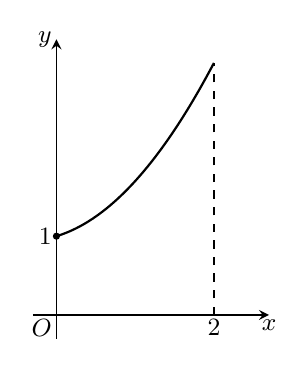
\begin{tikzpicture}[semithick, every node/.style={inner sep=1.4pt, font=\small}]
  \draw[-stealth] (-0.3,0) -- (2.7,0) node[below] {$x$};
  \draw[-stealth] (0,-0.3) -- (0,3.5) node[left] {$y$};
  \node[below left] at (0,0) {$O$};
  \fill (0,1) circle (1.3pt);
  \node[left] at (0,1) {$1$};
  \draw[thick,domain=0:2,samples=80] plot (\x,{1+0.30*\x+0.40*\x*\x});
  \draw[dashed] (2,0) -- (2,{1+0.30*2+0.40*4});
  \node[below] at (2,0) {$2$};
\end{tikzpicture}
\end{center}
\nopagebreak[4]
（A）$y=x^2+1$

（B）$y=|x|+1$

（C）$y=\begin{cases}2x+1,&x\geqslant0,\\ x^3+1,&x<0\end{cases}$

（D）$y=\begin{cases}\mathrm e^x,&x\geqslant0,\\ \mathrm e^{-x},&x<0\end{cases}$

\end{question}
\endgroup
\begin{question}
\gkti{9}在平面直角坐标系中，若不等式组 $\begin{cases}x+y-1\geqslant0,\\ x-1\leqslant0,\\ ax-y+1\geqslant0\end{cases}$（$a$ 为常数）所表示的平面区域内的面积等于 $2$，则 $a$ 的值为（　）

（A）$-5$

（B）$1$

（C）$2$

（D）$3$

\end{question}
\begin{question}
\gkti{10}设 $m$，$n$ 是平面 $\alpha$ 内的两条不同直线，$l_1$，$l_2$ 是平面 $\beta$ 内的两条相交直线，则 $\alpha\parallel\beta$ 的一个充分而不必要条件是（　）

（A）$m\parallel\beta$ 且 $l_1\parallel\alpha$

（B）$m\parallel l_1$ 且 $n\parallel l_2$

（C）$m\parallel\beta$ 且 $n\parallel\beta$

（D）$m\parallel\beta$ 且 $n\parallel l_2$

\end{question}
\begin{question}
\gkti{11}函数 $f(x)$ 的零点与 $g(x)=4^x+2x-2$ 的零点之差的绝对值不超过 $0.25$，则 $f(x)$ 可以是（　）

（A）$f(x)=4x-1$

（B）$f(x)=(x-1)^2$

（C）$f(x)=\mathrm e^x-1$

（D）$f(x)=\ln\left(x-\dfrac12\right)$

\end{question}
\begin{question}
\gkti{12}设 $\boldsymbol a$，$\boldsymbol b$，$\boldsymbol c$ 为同一平面内具有相同起点的任意三个非零向量，且满足 $\boldsymbol a$ 与 $\boldsymbol b$ 不共线，$\boldsymbol a\perp\boldsymbol c$，$|\boldsymbol a|=|\boldsymbol c|$，则 $|\boldsymbol b\cdot\boldsymbol c|$ 的值一定等于（　）

（A）以 $\boldsymbol a$，$\boldsymbol b$ 为邻边的平行四边形的面积

（B）以 $\boldsymbol b$，$\boldsymbol c$ 为邻边的平行四边形的面积

（C）以 $\boldsymbol a$，$\boldsymbol b$ 为两边的三角形面积

（D）以 $\boldsymbol b$，$\boldsymbol c$ 为两边的三角形面积

\end{question}
\gkpart{二、填空题}

\begin{question}
\gkti{13}复数 $\mathrm i^2(1+\mathrm i)$ 的实部是$\underline{\qquad}$．

\end{question}
\begin{question}
\gkti{14}点 $A$ 为周长等于 $3$ 的圆周上的一个定点．若在该圆周上随机取一点 $B$，则劣弧 $\overset{\frown}{AB}$ 的长度小于 $1$ 的概率为$\underline{\qquad}$．

\end{question}
\begin{question}
\gkti{15}若曲线 $f(x)=ax^2+\ln x$ 存在垂直于 $y$ 轴的切线，则实数 $a$ 的取值范围是$\underline{\qquad}$．

\end{question}
\begin{question}
\gkti{16}五位同学围成一圈依序循环报数，规定：

① 第一位同学首次报出的数为 $1$，第二位同学首次报出的数也为 $1$，之后每位同学所报出的数都是前两位同学所报出的数之和；

② 若报出的数为 $3$ 的倍数，则报该数的同学需拍手一次．

当第 $30$ 个数被报出时，五位同学拍手的总次数为$\underline{\qquad}$．

\end{question}
\gkpart{三、解答题}

\begin{question}
\gkti{17}等比数列 $\{a_n\}$ 中，已知 $a_1=2$，$a_4=16$．

（1）求数列 $\{a_n\}$ 的通项公式；

（2）若 $a_3$，$a_5$ 分别为等差数列 $\{b_n\}$ 的第 $3$ 项和第 $5$ 项，试求数列 $\{b_n\}$ 的通项公式及前 $n$ 项和 $S_n$．

\end{question}
\begin{question}
\gkti{18}袋中有大小、形状相同的红、黑球各一个，现一次有放回地随机摸取 $3$ 次，每次摸取一个球．

（1）试问：一共有多少种不同的结果？请列出所有可能的结果；

（2）若摸到红球时得 $2$ 分，摸到黑球时得 $1$ 分，求 $3$ 次摸球所得总分为 $5$ 的概率．

\end{question}
\begin{question}
\gkti{19}已知函数 $f(x)=\sin(\omega x+\varphi)$，其中 $\omega>0$，$|\varphi|<\dfrac\pi2$．

（1）若 $\cos\dfrac\pi4\cos\varphi-\sin\dfrac{3\pi}4\sin\varphi=0$，求 $\varphi$ 的值；

（2）在（1）的条件下，若函数 $f(x)$ 的图象的相邻两条对称轴之间的距离等于 $\dfrac\pi3$，求函数 $f(x)$ 的解析式；并求最小正实数 $m$，使得函数 $f(x)$ 的图象左平移 $m$ 个单位所对应的函数是偶函数．

\Needspace{0.4\textheight}
\end{question}
\begingroup
\renewenvironment{question}{\Needspace{0.5\textheight}}{}
\begin{question}
\gkti{20}如图，平行四边形 $ABCD$ 中，$\angle DAB=60^\circ$，$AB=2$，$AD=4$．将 $\triangle CBD$ 沿 $BD$ 折起到 $\triangle EBD$ 的位置，使平面 $EDB\perp$ 平面 $ABD$．

（1）求证：$AB\perp DE$；

（2）求三棱锥 $E-ABD$ 的侧面积．
\nopagebreak[4]
\begin{center}% 2009 年福建卷文科第 20 题：折叠后的三棱锥 E-ABD。
% 来源 PDF：普通高考/2009/2009福建文.pdf，SHA-256 f0a5111a6f86f4d4e8618c5c2cd0ecfd678a590b36ecbd033bb63b189700a0bc。
% 原页：第 1 页（A3 三栏）第 3 栏中部，书页码 517。
% 重绘依据：按折叠后 ED⊥平面 ABD 的构型重绘；B 在左下、D 在右下、A 在左上、E 在右上。
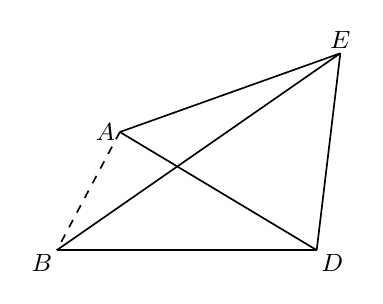
\begin{tikzpicture}[semithick, every node/.style={inner sep=1.4pt, font=\small}]
  \coordinate (B) at (0.0,0.0);
  \coordinate (D) at (3.3,0.0);
  \coordinate (A) at (0.8,1.5);
  \coordinate (E) at (3.6,2.5);
  % 可见棱
  \draw (E) -- (A);
  \draw (E) -- (B);
  \draw (E) -- (D);
  \draw (A) -- (D);
  \draw (B) -- (D);
  % 被遮挡的棱
  \draw[dashed] (A) -- (B);
  % 标注
  \node[left] at (A) {$A$};
  \node[below left] at (B) {$B$};
  \node[below right] at (D) {$D$};
  \node[above] at (E) {$E$};
\end{tikzpicture}
\end{center}
\nopagebreak[4]
\end{question}
\endgroup
\begin{question}
\gkti{21}已知函数 $f(x)=\dfrac13x^3+ax^2+bx$，且 $f'(-1)=0$．

（1）试用含 $a$ 的代数式表示 $b$；

（2）求 $f(x)$ 的单调区间；

（3）令 $a=-1$，设函数 $f(x)$ 在 $x_1$，$x_2$（$x_1<x_2$）处取得极值，记点 $M(x_1,f(x_1))$，$N(x_2,f(x_2))$．证明：线段 $MN$ 与曲线 $f(x)$ 存在异于 $M$、$N$ 的公共点．

\Needspace{0.4\textheight}
\end{question}
\begingroup
\renewenvironment{question}{\Needspace{0.5\textheight}}{}
\begin{question}
\gkti{22}已知直线 $x-2y+2=0$ 经过椭圆 $C:\dfrac{x^2}{a^2}+\dfrac{y^2}{b^2}=1$（$a>b>0$）的左顶点 $A$ 和上顶点 $D$，椭圆 $C$ 的右顶点为 $B$，点 $S$ 和椭圆 $C$ 上位于 $x$ 轴上方的动点，直线 $AS$，$BS$ 与直线 $l:x=\dfrac{10}3$ 分别交于 $M$，$N$ 两点．

（1）求椭圆 $C$ 的方程；

（2）求线段 $MN$ 的长度的最小值；

（3）当线段 $MN$ 的长度最小时，在椭圆 $C$ 上是否存在这样的点 $T$，使得 $\triangle TSB$ 的面积为 $\dfrac15$？若存在，确定点 $T$ 的个数，若不存在，说明理由．
\nopagebreak[4]
\begin{center}% 2009 年福建卷文科第 22 题：椭圆 x^2/4+y^2=1、直线 l:x=10/3 与点 A、B、S、M、N。
% 来源 PDF：普通高考/2009/2009福建文.pdf，SHA-256 f0a5111a6f86f4d4e8618c5c2cd0ecfd678a590b36ecbd033bb63b189700a0bc。
% 原页：第 2 页（A3 三栏）第 3 栏上部，书页码 518。
% 重绘依据：取 |MN| 最小时的 S(6/5,4/5)，M(10/3,4/3)、N(10/3,-4/3)。
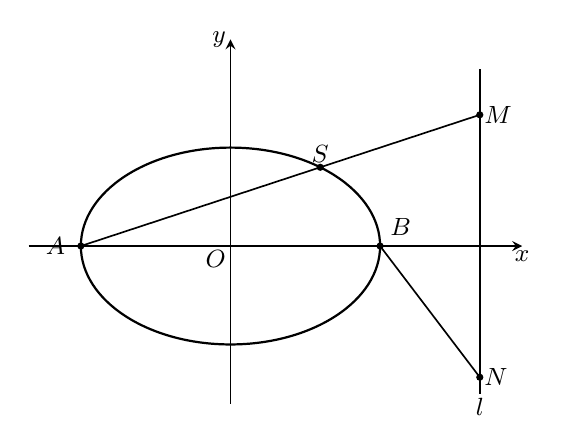
\begin{tikzpicture}[semithick, x=0.95cm, y=1.25cm, every node/.style={inner sep=1.4pt, font=\small}]
  % 坐标轴
  \draw[-stealth] (-2.7,0) -- (3.9,0) node[below] {$x$};
  \draw[-stealth] (0,-1.6) -- (0,2.1) node[left] {$y$};
  \node[below left] at (0,0) {$O$};

  % 椭圆
  \draw[thick] (0,0) ellipse (2 and 1);

  % 直线 l
  \draw (3.333,-1.5) -- (3.333,1.8);
  \node[below] at (3.333,-1.5) {$l$};

  % 点
  \coordinate (A) at (-2,0);
  \coordinate (B) at (2,0);
  \coordinate (S) at (1.2,0.8);
  \coordinate (M) at (3.333,1.333);
  \coordinate (N) at (3.333,-1.333);
  \fill (A) circle (1.3pt);
  \fill (B) circle (1.3pt);
  \fill (S) circle (1.3pt);
  \fill (M) circle (1.3pt);
  \fill (N) circle (1.3pt);

  % 直线
  \draw (A) -- (M);
  \draw (B) -- (N);

  % 标注
  \node[left=4pt] at (A) {$A$};
  \node[above right=2pt] at (B) {$B$};
  \node[above] at (S) {$S$};
  \node[right] at (M) {$M$};
  \node[right] at (N) {$N$};
\end{tikzpicture}
\end{center}
\nopagebreak[4]

\end{question}
\endgroup